%2S тут нужно проставить литературу - список литературы дан после каждой подсекции
\subsection{Совместное влияние аминокислотной последовательности гистона H1 и нуклеотидной последовательности ДНК на структуру хроматосомы: анализ методами молекулярного моделирования}

\textit{Текст ниже приведен согласно статье \cite{gorkovets_joint_2018} <<}

Хроматосома, состоящая из нуклеосомного ядра, линкерных участков ДНК и линкерного гистона H1 (ЛГ), является важным структурным элементом хроматина. Существует два экспериментально подтвержденных типа связывания ЛГ с нуклеосомой и линкерной ДНК, которые различаются своей геометрией - связывание ``на диаде'' и ``вне диады''. Показано, что на тип связывания гистона и конформацию хроматосомы влияет аминокислотная последовательность ЛГ.  Однако, при связывании ЛГ изменяется в том числе и геометрия линкерной ДНК. Взаимовлияние этих факторов и молекулярные основы, определяющие тип связывания ЛГ и нуклеосомы, остаются неясными. В данной работе мы применили методы молекулярного моделирования, включая моделирование по гомологии, анализ атом-атомных взаимодействий и расчет энергии деформации ДНК для изучения совместного влияния аминокислотной последовательности ЛГ и нуклеотидной последовательности ДНК на конфигурацию хроматосомы. Были проанализированы известные кристаллические и ЯМР структуры хроматосомы на предмет атом-атомных взаимодействий ЛГ и ДНК, а также энергии деформации ДНК в этих структурах для различных последовательностей ДНК. Для различных вариантов ЛГ анализ проводился с использованием методов моделирования по гомологии. Были обнаружены зависящие от последовательности различия в энергии изгиба линкерной ДНК для двух различных конформаций хроматосомы, а также предложены нуклеотидные последовательности, предпочтительные для этих структур. В результате анализа было показано, что нуклеотидная  последовательность ДНК наряду с аминокислотной последовательностью ЛГ оказывает влияние на тип связывания с нуклеосомой. Сформулированы гипотезы для экспериментальной проверки, согласно которым тип связывания ЛГ может меняться при изменении нуклеотидной последовательности ДНК. 

Структурными единицами хроматина являются нуклеосомы - ДНК-белковые комплексы, содержащие гистоны. Ядро нуклеосомы образовано октамером гистонов H2A, H2B, H3 и Н4, вокруг которого располагается двойная спираль ДНК длиной около 146 пар оснований \cite{luger_crystal_1997}. Нуклеосома обладает осью псевдосимметрии второго порядка, называемой также диадной осью (рисунок \ref{fig:p6_5_f1}А). Эта ось проходит через центр нуклеосомальной ДНК, называемый диадой.
Следующим уровнем компактизации является хроматосома \cite{simpson_structure_1978}, образованная при связывании линкерного гистона H1 (ЛГ) и нуклеосомы, включающей линкерные участки ДНК, выходящие за пределы ядра нуклеосомы (рисунок \ref{fig:p6_5_f1}А). Таким образом, в хроматосому входит октамер гистонов H2A, H2B, H3 и Н4, нуклеосомальная ДНК, ЛГ  и линкерные участки ДНК. 
ЛГ представлены во многих эукариотических организмах несколькими вариантами, различающимися длиной аминокислотной последовательности и ее составом \cite{lyubitelev_structure_2016}. В различных клетках и тканях могут экспрессироваться различные варианты ЛГ. Как правило, у наиболее просто устроенных организмов встречается всего один вариант ЛГ, тогда как, например, у человека известно 11 вариантов \cite{el_kennani_ms_histonedb_2017}, некоторые из которых экспрессируются только в половых клетках. Также стоит отметить, что присутствие того или иного варианта ЛГ зависит не только от типа клетки, но и от стадии клеточного цикла, в которой она находится.
Большая часть ЛГ содержит около 200 аминокислотных остатков. ЛГ состоят из трех доменов: короткий и неупорядоченный N-конец, за которым идет глобулярный домен, образованный 70-80 аминокислотными остатками и имеющий консервативную третичную структуру, и длинный С-концевой домен из примерно 100 аминокислотных остатков. С-конец является неорганизованным и содержит много остатков лизина. Согласно экспериментальным данным \cite{syed_single-base_2010} глобулярный домен ЛГ связывается с нуклеосомой наравне с полноразмерным ЛГ. Ввиду большой степени неупорядоченности концевых доменов отсутствуют кристаллические структуры полноразмерного ЛГ, но существуют кристаллические структуры глобулярного домена \cite{ramakrishnan_crystal_1993}.
В данный момент областью для обсуждений является конфигурация связывания ЛГ с нуклеосомой. Ранее существовали различные модели связывания ЛГ с нуклеосомой. Некоторые из них даже предполагали встраивание ЛГ между витками нуклеосомальной ДНК и октамером гистонов \cite{pruss_asymmetric_1996}. Подобные модели не нашли впоследствии экспериментального подтверждения \cite{syed_single-base_2010,zhou_position_1998} в отличие от моделей, в которых предполагается связывание ЛГ в области диады нуклеосомы и линкерных участков ДНК. 
Имеющиеся на текущий момент экспериментальные данные \cite{bednar_structure_2017,zhou_structural_2013,zhou_structural_2015,zhou_small_2016} предполагают два возможных расположения ЛГ в хроматосоме, условно называемые как «на диаде» (НД, ``on-dyad'') и «вне диады» (ВД, ``off-dyad''). На данный момент получена кристаллическая структуры хроматосомы с глобулярным доменом ЛГ H5 \textit{G. gallus} (H5 является историческим названием ЛГ Н1 у \textit{G. gallus}) в конфигурации НД, а также модель структуры хроматосомы с глобулярным доменом ЛГ Н1 \textit{D. melanogaster} в конфигурации ВД \cite{zhou_structural_2015}. Важно отметить, что структура хроматосомы в конфигурации ВД была построена с помощью методов молекулярного докинга на основании структуры тетрануклеосомы (pdb-код 1zbb) на основании данных ЯМР. 
Известно, что ЛГ содержит ряд аминокислотных остатков, играющих важную роль в формировании контактов с нуклеосомой \cite{brown_mapping_2006}. Эти остатки выделены в два сайта связывания: первый - H25, R47, K69, K73, R74, K85, и второй - R42, R94, K97.
Глобулярный домен гистона Н5 \textit{G. gallus} продемонстрировал связывания типа НД с нуклеосомой, тогда как глобулярный домен Н1 \textit{D. melanogaster} продемонстрировал связывание типа ВД. Анализ их последовательностей показал отличия, вероятно играющие роль в предпочтительности того или иного типа связывания. Так, глобулярный домен Н5 содержит положительно заряженные аминокислотные остатки (R47, K55, R74, K97) в позициях соответствуюих нейтрально заряженным аминокислотным остаткам в глобулярном домене Н1 (L68, T76, S96, A119), и нейтрально заряженные аминокислотные остатки (Q51, V80, V87) в позициях соответствующим положительно заряженным остатками Н1 (K72, K102, K109) \cite{zhou_structural_2015,zhou_small_2016}. Несмотря на то, что некоторые из ключевых остатков не образуют прямых контактов с нуклеосомой, при их замене в глобулярном домене Н5 на аминокислотные остатки, характерные для Н1, ЛГ показал изменение типа связывания с НД на ВД \cite{zhou_small_2016}.
Другим фактором, который предположительно может оказывать влияние на конфигурацию хроматосомы, является нуклеотидная последовательность ДНК, как линкерной, так и входящей в состав нуклеосомы. По данным исследования позиционирования нуклеосом выдвигались предположения, что ЛГ предпочтительно связывается с АТ-богатыми участками ДНК \cite{cui_distinctive_2009}. 
Несмотря на то, что в полученной кристаллической структуре хроматосомы ЛГ показал связывания НД, по данным, полученным методами молекулярного моделирования \cite{ozturk_conformational_2016,pachov_structure_2011}, глобулярный домен ЛГ Н5 может также демонстрировать тип связывания ВД. Одним из объяснений может служить тот факт, что нуклеотидные последовательности ДНК, используемые при моделировании, отличались от нуклеотидной последовательности, для которой была разрешена кристаллическая структура НД конформации комплекса нуклеосомы с глобулярным доменом Н5 \cite{zhou_structural_2015}.
В описанных выше работах рассматривается связывание ЛГ с одиночной нуклеосомой in vitro, тогда как в клетке представлены структуры более высокого уровня компактизации - 30 нм фибриллы, представляющей собой цепочку из нуклеосом и ЛГ, связанных с линкерной ДНК. Согласно последним данным крио-электронной микроскопии в структуре 30 нм фибриллы, образованной 12 нуклеосомами, ЛГ демонстрирует связывание ВД, что может быть обусловлено геометрией линкерной ДНК в структуре фибриллы \cite{bednar_structure_2017,song_cryo-em_2014}. Таким образом нельзя исключать влияние ДНК, вызванное ``узнаванием'' ЛГ специфической формы ДНК при связывании \cite{rohs_origins_2010}. 
Исходя из вышесказанного, весьма вероятно, что на тип связывания ЛГ с нуклеосомой и линкерной ДНК влияет не только аминокислотная последовательность самого гистона, но и нуклеотидная последовательность ДНК, а также структура хроматиновой фибриллы. Известно также, что при образовании комплекса белок-ДНК на силу и тип связывания оказывают влияние как прямые взаимодействия белка с парами оснований и сахаро-фосфатным остовом, так и геометрия ДНК за счет энергии ее деформации \cite{rohs_origins_2010}. Однако, несмотря на наличие структур хроматосомы в различных конфигурациях совместное влияние этих факторов ранее не изучалось.
В данной работе методами молекулярного моделирования, а именно анализа атом-атомных взаимодействий, моделирования по гомологии и оценки энергии деформации ДНК, было проведено изучение совместного влияния аминокислотной последовательности ЛГ и нуклеотидной последовательности ДНК на тип конфигурации хроматосомы. Проведенный анализ позволил предсказать наиболее предпочтительные для того или иного типа связывания нуклеотидные последовательности линкерной ДНК и сформулировать гипотезы для экспериментальной проверки.
\subsubsection{Материалы и методы}
\emph{Анализ аминокислотных последовательностей различных гистоновых вариантов}
В работе были использованы аминокислотные последовательности ЛГ, размещенные в базе данных HistoneDB \cite{draizen_histonedb_2016}. Выравнивание доступных аминокислотных последовательностей проводилось программой Muscle \cite{edgar_muscle_2004}. Для дальнейшего анализа последовательностей использовался biopython.
\emph{Моделирование по гомологии}
Моделирование по гомологии осуществлялось в программе MODELLER \cite{webb_comparative_2016,marti-renom_comparative_2000}. В качестве белков-шаблонов использовались кристаллическая структура хроматосомы в конфигурации НД с pdb-кодом 4qlc и модель хроматосомы в конфигурации ВД, полученная на основании данных ЯМР\cite{zhou_structural_2015}. Для каждого исследуемого гистона с помощью моделирования по гомологии было построено по 10 моделей, из которых на основании DOPEscore были отобраны наилучшие структуры для анализа контактов. Анализ контактов проводился с помощью программного пакета Chimera \cite{pettersen_ucsf_2004}.
\emph{Расчет энергии деформации ДНК}
Расчет зависимости деформационной энергии линкерных участков ДНК от ее последовательности производили в пространстве обобщенных переменных Tilt, Roll, Twist, Shift, Slide, Rise; переход от атомных координат к обобщенным осуществляли при помощи программы 3DNA \cite{lu_3dna_2003}. Вычисление деформационной энергии участков ДНК производили в соответствии с формулой (\ref{DNA_ener}). Для расчетов применяли набор упругих коэффициентов и средних значений для нуклеотидных пар описанный в работе \cite{olson_dna_1998}.  
Деформационную энергию определяли для всех возможных последовательностей ДНК для четырех участков ДНК (по два на каждую модель связывания ЛГ) длиной по 12 н.п. каждый. Участок ДНК, рядом с которым располагается линкерный гистон в модели ВД был назван входом в последовательность, позиционирующую нуклеосомы (ППН), противоположный участок был назван выходом из ППН. Для каждого варианта последовательности была рассчитана разница в деформационной энергии ДНК между моделями НД и ВД. Полученное распределение разниц энергий визуализировали при помощи графического представления консервативности нуклеотидов - логотипа последовательности (sequence logo) для 5% структур с наиболее положительной разницей энергий (предпочтительные для модели НД) и 5% структур с наиболее отрицательной разницей энергий (предпочтительные для модели ВД).
\subsubsection{Результаты и обсуждение}
Настоящее исследование состояло из нескольких взаимодополняющих компонент. На основе анализа экспериментальных данных были выделены ключевые остатки ЛГ, способствующие тому или иному типу связывания, на основании которых была построена классификационная модель, которая была применена к ЛГ человека: H1.1, H1.2, H1.3, H1.4, H1.5, H1.0 (H1$^\circ$), TS H1.6 (H1T), TS H1.7 (H1T2, HANP1), OO H1.8 (H1oo), TS H1.9 (HILS1), H1.10, H1.11, а также к ЛГ \textit{X. laevis}. Для экспериментально определенных структур хроматосомы и структур с различными вариантами ЛГ, построенных с помощью моделирования по гомологии были проанализированы контакты между ЛГ и ДНК. Был проведен оригинальный анализ конформации ДНК в различных структурах хроматосомы и анализ пространства последовательностей линкерных ДНК с точки зрения энергии их изгиба и контактов с ЛГ. 

\emph{Определение ключевых остатков ЛГ, влияющих на тип связывания}
Аминокислотная последовательность ЛГ имеет ряд ключевых позиций, мутации в которых приводят к изменению типа связывания \cite{zhou_small_2016}. Таким образом, на основании аминокислотных остатков, расположенных в этих позициях, для ЛГ может быть определен предполагаемый тип связывания, что позволяет предложить классификацию ЛГ по типу их связывания с нуклеосомой на основании аминокислотных последовательностей. 
В экспериментально определенной структуре хроматосомы в конфигурации НД и ВД присутствуют контакты непосредственно с парами оснований и линкерной ДНК, и нуклеосомальной ДНК, данные взаимодействия представлены как водородными связями, так и Ван-дер-Ваальсовыми взаимодействиями. 
Некоторые из аминокислотных остатков, расположенных в ключевых позициях (например, аминокислотные остатки, соответствующие K55, Q51, V87 ЛГ Н5) не образуют прямых контактов с ДНК в известных структурах. Однако, несмотря на отсутствие контактов с ДНК, данные остатки предположительно могут взаимодействовать с ДНК посредством электростатического потенциала, поскольку в гистонах Н1 и Н5 они имеют различные заряды.
\emph{Классификация ЛГ на основании наличия ключевых остатков}
На основании предложенной выше классификации, было показано, что для 3 ЛГ человека предполагаемый тип связывания был определен как НД, для 7 гистонов человека тип связывания не может быть определен однозначно, поскольку они демонстрируют сходство в ключевых позициях и с гистоном Н5 \textit{G. gallus} (тип связывания НД), и с гистоном Н1 \textit{D. melanogaster} (тип связывания ВД), для 1 гистона человека предполагаемый тип связывания может быть определен однозначно как ВД. Для ЛГ \textit{X. laevis} тип связывания был определен как НД. 

   \begin{figure} [H]
    \centering
    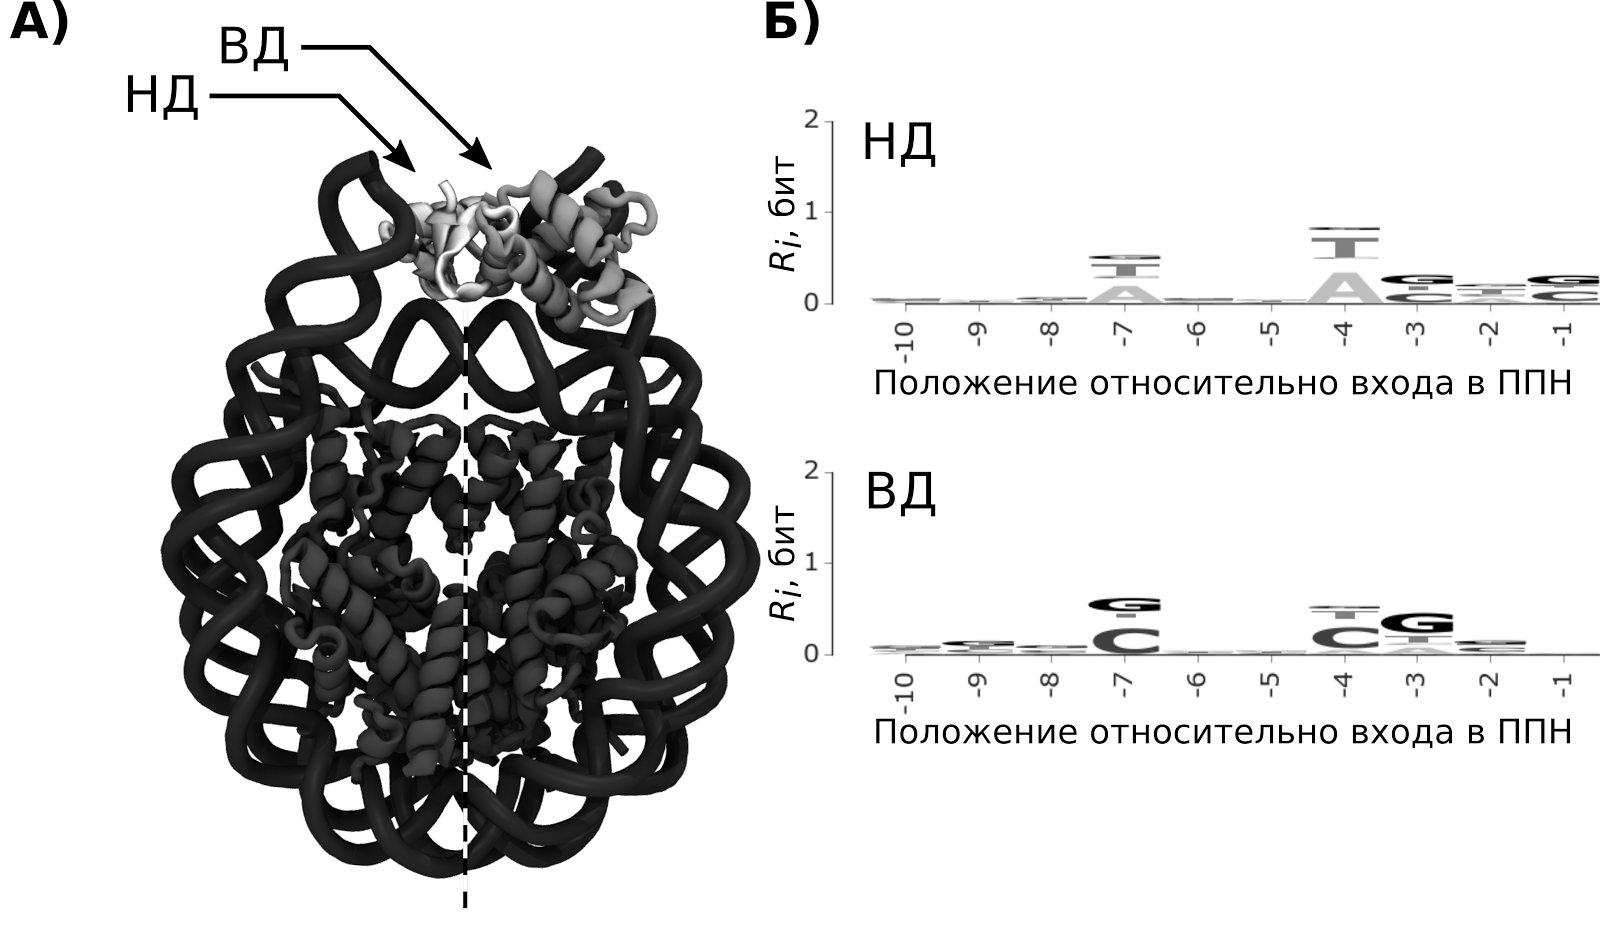
\includegraphics[width=\textwidth]{images/p6/p6_5/p6_5_f1.png}
    \caption[Cтруктура хроматосомы и оптимальные последовательности линкерной ДНК.]{Cтруктура хроматосомы и оптимальные последовательности линкерной ДНК. A) Внешний вид структуры хроматосомы. Белок и ДНК показаны в виде отображения вторичной структуры. Линкерные гистоны выделены оттенками серого. Диадная ось показана пунктирной линией.
Б) Визуализация частоты встречаемости нуклеотидов для последовательностей, склонных к формированию структуры НД (сверху) и ВД (снизу). Визуализация выполнена в виде логотипов последовательностей.
}
    \label{fig:p6_5_f1}
\end{figure}

\emph{Энергия деформации ДНК в различных конфигурациях хроматосомы}
Для определения зависимости типа связывания ЛГ от нуклеотидной последовательности линкерной ДНК была рассчитана разница деформационных энергий линкерных участков ДНК между моделями НД и ВД для всех возможных вариантов последовательностей. Также была произведена Z-оценка положения последовательности из оригинальных моделей в распределении рассчитанных деформационных энергий (Z=0,75), исходя из которой оригинальная последовательность, использованная для экспериментального получения структур, склонна к формированию структуры НД.
Как видно из рисунка \ref{fig:p6_5_f1}Б, большинство позиций в последовательностях нуклеотидов линкерных участков ДНК не значимы для определения геометрии ДНК в рамках моделей НД и ВД, кроме нуклеотидов в позициях -7, -4 и -3. В последовательностях, предпочтительных для модели НД, в этих позициях располагаются A/T, A/T, G/C, в то время как для модели ВД более предпочтительны  C/G, C/T, G/T. Богатость линкерной ДНК тимидинами также была показана в работе \cite{cui_distinctive_2009}.
Также по разнице в деформационных энергиях были найдены предпочтительные (оптимальные) последовательности линкерной ДНК (для которых энергия изгиба максимально способствует той или иной конформации) для моделей НД (CCGTCCCGTC-ППН-ACGCCGGCGG) и ВД (GACGCCCGAC-ППН-GTGATGCTGC). 

\emph{Анализ совместного влияния аминокислотной последовательности ЛГ и нуклеотидной последовательности ДНК}
На основании предложенной ранее классификации для различных вариантов ЛГ с помощью моделирования по гомологии были построены структурные модели хроматосом в конфигурациях НД и ВД. В полученных моделях был проведен анализ контактов между ЛГ и ДНК.
И в тех, и в других моделях присутствуют контакты как между аминокислотными остатками ЛГ и сахаро-фосфатным остовом ДНК, так и непосредственно с азотистыми основаниями, что говорит в пользу предположений о том, что нуклеотидная последовательность ДНК может оказывать влияние на тип связывания ЛГ и нуклеосомы за счет эффекта прямого считывания последовательности ДНК белком (direct readout). Также количество этих контактов изменяется в зависимости от варианта ЛГ, для которого построена модель. Взаимодействия между ЛГ и азотистыми основаниями ДНК могут быть, как водородными связями, так и ван-дер-Ваальсовыми взаимодействиями. 
Также для ЛГ Н1 \textit{D. melanogaster} и Н5 \textit{G. gallus} с помощью моделирования по гомологии были построены модели хроматосом в конфигурациях, противоположных экспериментальным: для ЛГ Н1 использовалась конфигурация НД, для ЛГ Н5 - конфигурация ВД. Данные модели показали уменьшение количества контактов между ЛГ и ДНК, что согласуется с определенными экспериментально типами связывания.
На основании расчета энергии деформации ДНК были построены модели хроматосомы в конфигурации НД и ВД с предпочтительными (оптимальными) для них последовательностями, определенными по разнице в энергии деформации ДНК, для которых также были проанализированы контакты между ЛГ и ДНК. Анализ показал, что при замене исходной нуклеотидной последовательности в экспериментальных структурах ВН и НД на оптимальные последовательности, способствующие исходному типу связывания, определенные в нашей работе, количество контактов ЛГ с парами оснований либо не меняется (ВД 3->3), либо увеличивается (НД 2->3). В то же время, перекрестное сравнение эффектов оптимальных последовательностей ДНК в НД и ВД структурах показало, что структуры с оптимальными последовательностями ДНК, соответствующими своему типу связывания имеют такое же или большее число контактов между ЛГ и парами оснований, чем структуры, в которых используется последовательность ДНК, соответствующая альтернативному типу связывания. Таким образом, оптимальные последовательности линкерной ДНК для различных конформаций хроматосомы, предложенные выше, могут достигать своей избирательности как за счет механизмов непрямого считывания  последовательности ДНК белком (indirect readout), так и прямого считывания (direct readout) - взаимодействие белка с парами оснований.
 Исходя из вышесказанного, можно сделать предположение, что нуклеотидная последовательность, а также геометрия и изгибная жесткость ДНК являются важным фактором определяющим тип конфигурации хроматосомы. Это предположение на данный момент согласуется косвенным образом с экспериментальными данными \cite{bednar_structure_2017,song_cryo-em_2014}. Вероятно, аминокислотная последовательность ЛГ не является первостепенным фактором определяющим тип связывания ЛГ с нуклеосомой.
Подводя итог, можно сформулировать гипотезу, согласно которой один и тот же ЛГ в зависимости от нуклеотидной последовательности ДНК, а также от геометрии линкерной ДНК, может показывать различные типы связывания. Такие пары последовательностей ДНК предложены в данной работе. В дальнейшем эта гипотеза может быть проверена путем оценки расстояний между нуклеотидами, методом измерения эффективности Фёрстеровского переноса энергии (spFRET), с использованием различных нуклеотидных последовательностей для каждого ЛГ.

\subsubsection{Благодарности}
Авторы выражают благодарность Y. Bai за предоставленную модель  хроматосомы. Работа выполнена с использованием оборудования Центра коллективного пользования сверхвысокопроизводительными вычислительными ресурсами МГУ имени М.В. Ломоносова \cite{voevodin_supercomputer_2019}. Работа выполнена при финансовой поддержке Российского научного фонда (проект №14-24-00031, соглашение №14-24-00031-п).
\textit{>>}



\subsection{Моделирование структуры ДНК в хроматосоме по данным FRET}

\textit{Текст ниже приведен согласно статье \cite{armeev_modeling_2016} <<}

В работе данного подраздела рассматриваются методы построения трехмерных моделей ДНК в комплексе с белками на основании компьютерного моделирования и непрямых методов изучения конформации макромолекул. Предложен алгоритм поиска конформации комплексов белков с ДНК на основе данных ферстеровского резонансного переноса энергии (FRET) и информации о локальной гибкости ДНК. Алгоритм апробирован на примере построения гипотетической модели ДНК в нуклеосоме при связывании гистона H1.


Структура ДНК-белковых комплексов влияет на течение множества процессов, таких как транскрипция, репликация и репарация. В исследованиях структуры додекамеров ДНК было показано, что ДНК значительно отличается от идеальной структуры двунитевой спирали. Необходимость существования более высоких уровней организации структуры ДНК очевидна, так как геном эукариотического организма не может разместиться в относительно компактном ядре в полностью развернутом виде. 
В 1974 году Р. Корнбергом \cite{kornberg_chromatin_1974} были открыты объекты - структурные единицы компактизации хроматина, которые позже были названы нуклеосомами. Структура нуклеосом долгое время оставалась неясной, и лишь в 1997 году методом рентгеноструктурного анализа (РСА) была определена первая структура нуклеосомы с почти атомарным разрешением \cite{luger_crystal_1997}. Нуклеосома представляет собой октамер белков гистонов, который несет на себе 145-147 нуклеотидных пар. ДНК закручена вокруг октамера, образуя 1,65 витка левозакрученной суперспирали. Белковое ядро нуклеосомы образует цилиндр диаметром 65 Å и высотой 60 Å. На уровне единичных нуклеосом происходит тонкая регуляция работы генетического аппарата клетки. Одним из ярких примеров регуляции экспрессии генов является так называемый нуклеосомальный барьер \cite{studitsky_overcoming_1995}: в зависимости от типа и структуры нуклеосомы, РНК полимераза II может иметь разную вероятность прохождения сквозь нуклеосому. Помимо этого, нуклеосомы взаимодействуют со множеством разнообразных транскрипционных факторов и структурных белков. Существует большое количество гистоновых вариантов, последовательность и структура которых отличается от канонических, что определяет их специфические свойства \cite{schalch_x-ray_2005}. Например, в областях центромер хромосом ДНК находится на специфических нуклеосомах, содержащих модифицированный гистон CenH3 (CENP-A). 
Нуклеосомы являются ключевыми и фундаментальными единицами упаковки ДНК, их взаимодействия, а также пространственная конфигурация хроматина определяют процессы реализации и передачи генетической информации. Изучение нуклеосом было сильно облегчено с появлением информации об их атомарном устройстве, и на данный момент в банке данных PDB насчитывается более 100 структур различных нуклеосом. Однако изучение более высоких уровней организации хроматина обычными методами структурной биологии затруднено. На данный момент, одной из крупнейших структур, полученной методом РСА, является комплекс из четырех нуклеосом \cite{schalch_x-ray_2005}. Хроматиновые фибриллы трудно изучать при помощи РСА, так как структуры такого размера крайне сложно кристаллизовать, к тому же места расположения нуклеосом не фиксированы строго \cite{mueller-planitz_nucleosome_2013}, а значит хромосомы в кристалле будут значительно отличаться друг от друга. Информацию о структуре можно получать косвенно биофизическими и биохимическими методами, например, методом ферстеровского резонансного переноса энергии (FRET) и методом футпринтинга ДНК. 
Метод FRET основан на явлении безизлучательного переноса энергии с одного красителя на другой. Красители подбирают таким образом, чтобы донор флуоресцировал в области спектра поглощения акцептора, и метят ими аминокислоты или азотистые основания ДНК. Вероятность переноса энергии значительно зависит от расстояния между флуоресцентными метками, таким образом, измеряя эффективность FRET можно оценить дистанцию между участками меченной макромолекулы. В работе \cite{falk_cenp-c_2015} таким методом были показаны тонкие различия (5 \AA) между канонической и центромерной нуклеосомой. Измерения FRET можно производить в растворе, при этом усредняется сигнал от всех, находящихся в нем молекул, но измерения такого рода не позволяют судить о конформационных переходах внутри исследуемых молекул. Помимо этого, измерения можно производить в режиме единичных молекул, собирая флуоресценцию лишь с малого конфокального объема в растворе. Такие измерения позволяют различать конформационные переходы в структуре молекул, определять заселенность разных конформаций а так же оценивать времена таких переходов. Таким образом, FRET позволяет получить набор расстояний между парами оснований в меченой макромолекуле. Комбинируя эту информацию с механическими свойствами ДНК можно судить о трехмерной структуре изучаемых комплексов.

Моделирование ДНК и нуклеосом можно производить в полноатомном разрешении \cite{shaytan_combined_2015} и рассчитывать энергию конформации ДНК при помощи традиционных силовых полей (AMBER, CHARMM и т.д.). Однако расчет энергии и поиск оптимальной конфигурации для таких моделей отличается высокой ресурсоемкостью. Для повышения скорости расчетов применяют огрубленные модели. В одной из таких моделей каждая нуклеотидная пара описывается шестью переменными (три трансляционных координаты и три вращательных), как и каждый шаг, между нуклеотидными парами \cite{dickerson_definitions_1989}. Таким образом для цепи из N нуклеотидных пар конфигурация ДНК описывается набором из 12N - 6 обобщенных переменных. Такой подход, в отличие от других огрубленных моделей позволяет однозначно воссоздавать атомарную структуру молекулярного комплекса. Дополнительно в данную модель модно ввести пространственные ограничения, полученные из экспериментов FRET, позволяя получить конфигурацию исследуемого объекта в атомарном разрешении. 
\subsubsection{Материалы и методы}
\emph{Интерпретация данных FRET одиночных молекул}
Расчет расстояний по данным FRET производился в соответствии с формулой (\ref{fret_E}). Ферстеровский радиус полагался равным 56\AA{} для пары меток Cy3/Cy5.
 Расстояние, рассчитанное для пары красителей, не соответствует расстоянию между нуклеотидными парами, так как метки закреплены на ДНК при помощи линкерного участка из 10-15 атомов углерода. Для учета смещения были созданы молекулярные модели меток. При помощи метода молекулярной динамики был построен набор их конформеров и определены координаты наиболее вероятного местонахождения меток. Моделирование производилось в программе Gromacs  \cite{abraham_gromacs:_2015} без учета электрических взаимодействий при температуре 500 K. Полученные координаты центров меток в дальнейшем использовались для расчета расстояния между нуклеотидными парами при оптимизации геометрии ДНК.

\emph{Расчет энергии деформации ДНК}
Энергия деформации рассчитывалась из обобщенных переменных, описывающих конфигурацию ДНК в соответствии с формулой (\ref{DNA_ener}). 
Коэффициенты жесткости ДНК для отклонения обобщенных переменных для каждой нуклеотидной пары взяты из работы \cite{olson_dna_1998}. Расчет обобщенных переменных из атомистической структуры и восстановление координат из набора переменных производился при помощи программы 3DNA \cite{lu_3dna_2003}. Минимизация энергии производилась по методу сопряженных градиентов. 
Все расчеты производились на персональном компьютере в программной среде python  с модулем scipy.

\subsubsection{Результаты и обсуждение}
Энергию изгиба ДНК можно рассчитывать при помощи силовых полей, которые применяют для моделирования методом молекулярной динамики, однако ресурсоемкость таких расчетов и проблемы с явным учетом электростатических взаимодействий ограничивают применение такого подхода. Другим способом расчета энергии деформации является применение набора эмпирических силовых коэффициентов, которые были получены путем анализа геометрии ДНК из множества различных кристаллических структур \cite{olson_dna_1998}.  Расчет конформации в обобщенных координатах можно производить быстрее, так как число переменных в модели значительно меньше. 
Так как минимизация происходит в пространстве обобщенных координат конформации ДНК, а расчет расстояний в трехмерном пространстве, на каждом шаге минимизации требуется производить расчет атомарной модели ДНК. Общий алгоритм поиска конфигурации ДНК, отвечающий критериям жесткости нуклеиновой кислоты, расстояниям, полученным из FRET, а также ограничениям, полученным из анализа профилей футпринтинга показан на рисунке \ref{fig:p6_5_f2}.

   \begin{figure} [H]
    \centering
    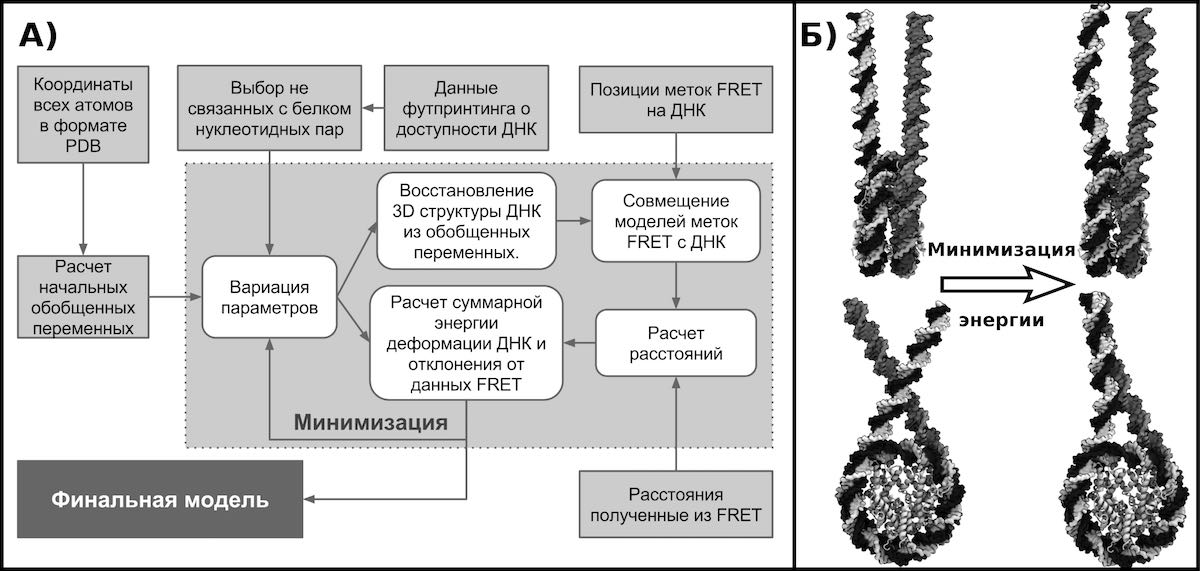
\includegraphics[width=\textwidth]{images/p6/p6_5/p6_5_f2.pdf}
    \caption[Создание моделей ДНК в хроматосоме по данным FRET.]{Создание моделей ДНК в хроматосоме по данным FRET. A) Схема алгоритма поиска конформации ДНК с учетом FRET и дригих данных. Пунктиром выделен блок минимизации энергии при поиске структур. Б) Визуализация результата поиска конформации хроматосомы. Гистоны отображены в виде вторичной структуры, ДНК показана в поверхности доступной растворителю.
}
    \label{fig:p6_5_f2}
\end{figure}

К недостаткам такого подхода можно отнести отсутствие учета взаимодействий между участками ДНК, что может привести к возникновению стерических перекрываний внутри молекулы. Однако при корректном выборе участков ДНК для минимизации, появление таких структур маловероятно.
В качестве объекта для испытания метода была использована нуклеосома с гистоном H1. Этот комплекс на момент проведения работы отсутствовал в банке трехмерных структур PDB, но были работы, где его структура исследуется при помощи ядерного магнитного резонанса \cite{zhou_structural_2013}. Гистон Н1, также называемый линкерным, образует комплекс с нуклеосомами, способствуя более высокому уровню компактизации ДНК. Оказывая такое влияние на размещение/упорядочение   ДНК в клетке, гистон Н1 играет большую роль в регуляции экспрессии генов. Структурные особенности взаимодействия линкерного гистона и нуклеосомы до сих пор неизвестны и их изучение вызывает большой интерес. 
За основу для построения модели была выбрана структура 1KX5 \cite{davey_solvent_2002} из банка данных PDB к которой были добавлены прямые линкеры в соответствии с последовательностью, что применялась в эксперименте FRET.  После проведения минимизации геометрии ДНК с ограничениями расстояний из данных FRET была получена асимметричная структура с параллельным расположением линкерных участков ДНК. Весьма схожие модели были получены в работе \cite{syed_single-base_2010}, где структуру хроматосом исследовали методом гидроксильного футпринтинга и электронной микроскопии. В дальнейшем полученная структура может быть применена в качестве мишени для макромолекулярного докинга гистона H1. 
Понимание молекулярных основ функционирования хроматина встречается с проблемами ограниченности экспериментальных методик в определении параметров взаимодействий ДНК с гистонами, транскрипционными факторами и структурными белками на молекулярном уровне. Данная проблема является следствием того, что экспериментальные методы вроде РСА, ЯМР и электронной микроскопии в состоянии определить структуры лишь небольших комплексов, которые обладают компактной и упорядоченной структурой. В то же время все больший интерес привлекают к себе структуры, не отличающиеся строгой упорядоченностью и их описание хроматина должно вестись не в рамках одиночных структур, а в рамках набора конформационных ансамблей.
Разработан метод, позволяющий создавать модели геометрии ДНК в комплексах с белками на основании интегрирования экспериментальных данных и данных о локальной жесткости ДНК при помощи молекулярного моделирования. Данный метод позволяет получать атомистические модели, позволяя изучать особенности комплексов как внутри, так и с другими. На примере хроматосомы показана возможность получения геометрии линкерной ДНК, что важно для понимания устройства хроматина. 
\emph{Благодарности}
Авторы работы выражают благодарность проф. В.М. Студитскому, проф. А.В.Феофанову и сотрудникам их лабораторий за предоставленные данные FRET.Данная работа выполнена при поддержке гранта Российского научного фонда (грант N14-24-00031).

\textit{>>}